\subsection{Background}

LCSs are surfaces of trajectories in a system that exert a major influence on nearby trajectories over time. The type of influence can vary (attracting, repelling, shearing) but they create a coherent trajectory pattern, for which the LCS can serve as a theoretical centerpiece \cite{Haller2000}.

In our case, individual ants act as the tracer particles, being carried by an underlying background flow. A \textit{dynamical system} in its most general form is -

\begin{equation}
    \left.
        \begin{array}{l}
            \dot{\vec{x}}(t;t_0,x_0) = \vec{v}(\vec{x}(t;t_0,\vec{x}_0),t) \, ,\\
            \vec{x}(t;t_0,\vec{x}_0) = \vec{x}_0 \, .
        \end{array}
    \right \}
    \label{eqn:dynamic}
\end{equation}

As time evolves, solutions of Equation \ref{eqn:dynamic} trace out curves in $D \subseteq \mathbb{R}^n$, or - they flow along their trajectory. If we fix the initial time $t_0$ and final time $t$, then we can define a flow map $\phi^t_{t_0}$ -

\begin{equation}
    \phi^t_{t_0} : D \rightarrow D : \vec{x}_0 \mapsto \phi^t_{t_0}(\vec{x}_0) = \vec{x}(t;t_0,\vec{x}_0)
\end{equation}

When analysing the phase space of these trajectories, we discover the notion of separatrices, which divide the flow into regions of distinct dynamics. For time dependent systems (as our ant model is likely to be), these separatrices themselves change with time. To find separatrices in time-dependent systems, one might look at fixed points of the instantaneous vector field and try to grow these manifolds by seeding near an instantaneous fixed point and advecting the points according to the time-dependent vector field. But separatrices in time-dependent flows aren't always connected to instantaneous fixed points, and hence we do an indirect study.

We do this by considering the behaviour of trajectories near these structures. Consider a a generic hyperbolic point and its associated stable and unstable manifolds, which is depicted in Fig. \ref{fig:hyperbolic}. If we integrate two points that are initially on either side of a stable manifold forward in time, then these points will eventually diverge from each other. Likewise, if we started two points on either side of an unstable manifold, then these points would quickly diverge from each other if integrated backward in time. This is why these manifolds are often called separatrices, since they separate trajectories which do qualitatively different things.

\begin{figure}
    \centering
    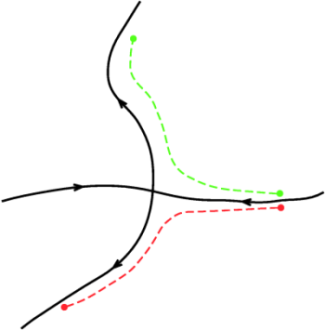
\includegraphics{figures/hyperbolic_point.png}
    \caption{Two points on either side of a separatrix will diverge from each other}
    \label{fig:hyperbolic}
\end{figure}

Therefore we take the viewpoint that since separatrices divide regions of qualitatively different dynamics, we can perhaps uncover or define such structures by looking at the divergence or stretching between trajectories. \cite{LCSTut}

\subsection{Finite-Time Lyapunov Exponents}

The finite-time Lyapunov exponent, FTLE, $\sigma_t^T(\vec{x})$, is a scalar value which characterizes the amount of stretching about the trajectory of point $\vec{x} \in D$ over the time interval $\left[t, t + T\right]$.

Consider two nearby points $\vec{x}$ and $\vec{y} = \vec{x} + \delta \vec{x}(t_0)$. After a time interval $T$, the separation between these points becomes -

\begin{align*}
    \delta \vec{x}(t_0 + T) & = \phi^{t_0 + T}_{t_0}(\vec{y}) - \phi^{t_0 + T}_{t_0}(\vec{x}) \\
    & = \frac{d\phi^{t_0 + T}_{t_0}(\vec{x})}{d\vec{x}}\delta \vec{x}(t_0) + \mathcal{O}(||\delta\vec{x}(t_0)||^2)
\end{align*}

The magnitude of perturbation is given by -

\begin{equation}
    ||\delta\vec{x}(t_0 + T)|| = \sqrt{\langle \delta\vec{x}(t_0) , \Delta \delta\vec{x}(t_0) \rangle}
\end{equation}

where, 
\begin{equation}
    \Delta = \left(\frac{d\phi^{t_0 + T}_{t_0}(\vec{x})}{d\vec{x}}\right)^*\left(\frac{d\phi^{t_0 + T}_{t_0}(\vec{x})}{d\vec{x}}\right)
\end{equation}

is a finite-time version of the Cauchy-Green deformation tensor. If we are interested in the maximum stretching occurring between points $\vec{x}$ and $\vec{y}$, we take $\delta \vec{x}(t_0)$ to be along the eigenvector associated with the maximum eigenvalue of $\Delta$. Assume $\lambda_{\text{max}}(\Delta)$ is the maximum eigenvalue, then -

\begin{equation}
    \text{max}||\delta\vec{x}(t_0 + T)|| = \sqrt{\lambda_{\text{max}}(\Delta)}||\delta\vec{x}(t_0)||
    \label{eqn:maxdelta}
\end{equation}

where $\delta\vec{x}(t_0)$ is aligned with the eigenvector described above. Define -

\begin{equation}
    \sigma_{t_0}^T(\vec{x}) = \frac{1}{|T|}\text{ln}\sqrt{\lambda_{\text{max}}(\Delta)}
\end{equation}

which makes equation \ref{eqn:maxdelta} look like 

\begin{equation}
    \text{max}||\delta\vec{x}(t_0 + T)|| = e^{\sigma_{t_0}^T(\vec{x})|T|}||\delta\vec{x}(t_0)||
\end{equation}

So, by analysing the flow of tracers placed on a uniform grid, one can obtain the FTLE associated with each point on the grid, which is what our ant simulations aim to do. FTLEs are critical in LCS analysis because separatrices are analogous to 'ridges' of high FTLE values in the FTLE field.

\subsection{FTLE fields for our model}

\begin{figure}
    \centering
    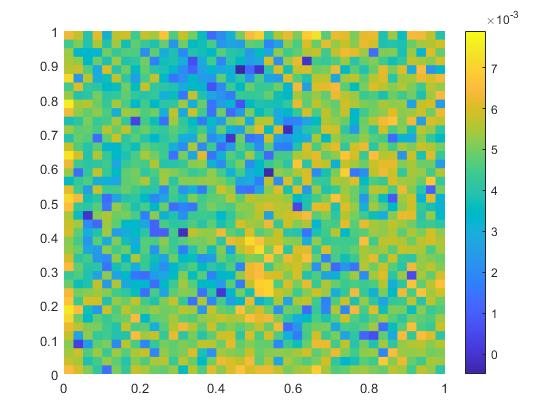
\includegraphics[scale = 0.35]{figures/FTLE_1.jpg}
    \caption{FTLE field for $t_0 = 0s, T = 20s$}
    \label{fig:ftle1}
\end{figure}

\begin{figure}
    \centering
    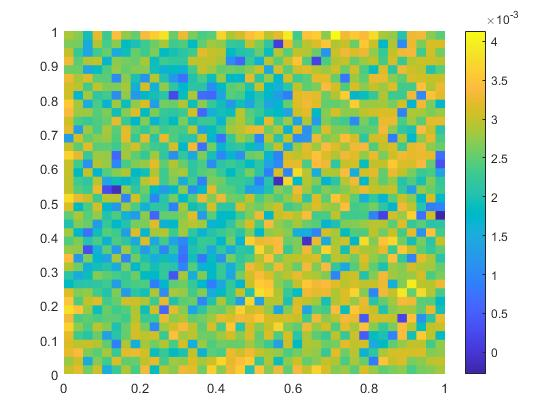
\includegraphics[scale = 0.35]{figures/FTLE_2.jpg}
    \caption{FTLE field for $t_0 = 0s, T = 40s$}
    \label{fig:ftle2}
\end{figure}

\begin{figure}
    \centering
    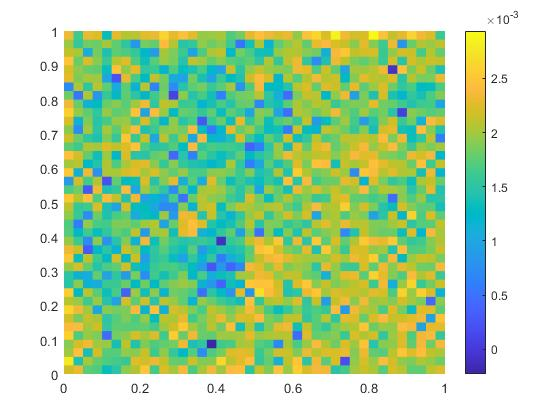
\includegraphics[scale = 0.35]{figures/FTLE_3.jpg}
    \caption{FTLE field for $t_0 = 0s, T = 60s$}
    \label{fig:ftle3}
\end{figure}

\begin{figure}
    \centering
    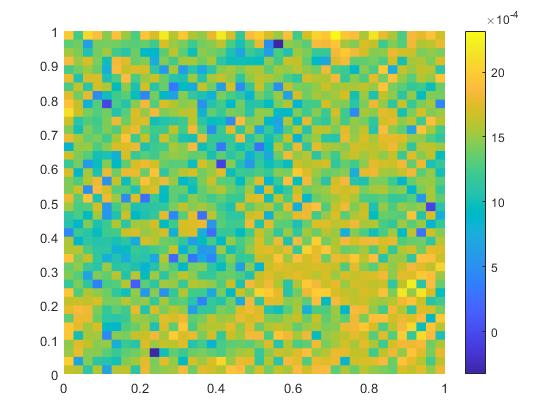
\includegraphics[scale = 0.35]{figures/FTLE_4.jpg}
    \caption{FTLE field for $t_0 = 0s, T = 80s$}
    \label{fig:ftle4}
\end{figure}

\begin{figure}
    \centering
    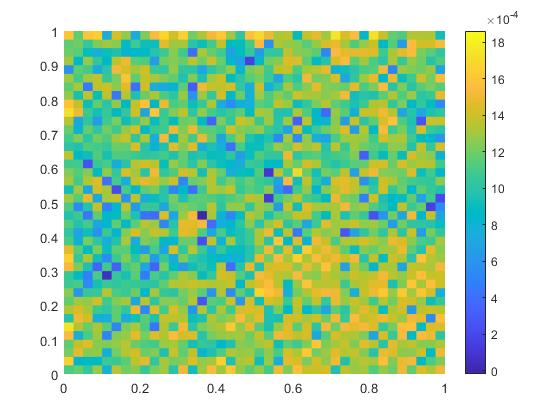
\includegraphics[scale = 0.35]{figures/FTLE_5.jpg}
    \caption{FTLE field for $t_0 = 0s, T = 100s$}
    \label{fig:ftle5}
\end{figure}

The defining characteristic of our simulations is lane formation and clumping of ants along these trails, which isn't something you readily see in the evolution of our FTLE fields. I suspect Backward-time FTLE fields will give us more stark separatrices that would correspond to our observed structures, and figuring out the best way to plot those across the entire grid is what I'm currently working on.

The figures for the FTLE fields for different values of $T$ are shown in Figures \ref{fig:ftle1}, \ref{fig:ftle2}, \ref{fig:ftle3}, \ref{fig:ftle4} and \ref{fig:ftle5}.